 \chapter{Análisis y documentación}
	 Este capítulo describe el proceso de adquisición de conocimientos necesarios para poder llevar a cabo el proceso de diseño arquitectónico y de construcción o implementacíon de la aplicación. De esta fomra se puede realizar una planificación mas cercana a la realidad y partir de unos conocimientos mínimos para empezar a elaborar el proyecto.
	 
	 \minitoc
	 
	 	\section{GO.JS}
	 		
	 		
	 		\begin{figure}[H]
	 			\centering
	 			
\includegraphics[scale=1]{gojs.jpeg}
	 			\caption{GO.JS Logo}\label{fig:gojs}
	 		\end{figure}
	 	
	 	
	 		\subsection{¿Qué es GO.JS?}
	 			Go.JS \cite{gojs} es una biblioteca de JavaScript con múltiples funciones para implementar diagramas interactivos personalizados y visualizaciones complejas en navegadores y plataformas web modernos.
	 	
	 		\subsection{¿Porqué GO.JS?}
	 		 GoJS facilita la construcción de diagramas de JavaScript de nodos, enlaces y grupos complejos con plantillas y diseños personalizables.
	 		
	 		
	 		\subsection{Características}
	 		GoJS ofrece muchas características avanzadas para la interactividad del usuario, tales como arrastrar y soltar, copiar y pegar, edición de texto en el lugar, información sobre herramientas, menús contextuales, diseños automáticos, plantillas, vinculación y modelos de datos, administración de estado transaccional y deshacer, paletas , vistas generales, controladores de eventos, comandos y un sistema de herramientas extensible para operaciones personalizadas.
	 		
	 	
	 		\subsection{Explicación}
	 		GoJS ofrece muchas características avanzadas para la interactividad del usuario, tales como arrastrar y soltar, copiar y pegar, edición de texto en el lugar, información sobre herramientas, menús contextuales, diseños automáticos, plantillas, vinculación y modelos de datos, administración de estado transaccional y deshacer, paletas , vistas generales, controladores de eventos, comandos y un sistema de herramientas extensible para operaciones personalizadas.
	 
	 
	 	\section{Vaadin}
	 	
	 		\begin{figure}[H]
	 			\centering
	 			
\includegraphics[scale=1]{Vaadin-logo.png}
	 			\caption{Vaadin Logo}\label{fig:Vaadin-logo}
	 		\end{figure}
 		
 			\subsection{¿Qué es GO.JS?}
 				Vaadin\cite{vaadin} es un framework de desarrollo de SPA que permite escribir el código de dichas aplicaciones en Java o en cualquier otro lenguaje soportado por la JVM 1.6+. Esto permite la programación de la interfaz gráfica en lenguajes como Java 8, Scala o Groovy, por ejemplo.
 			
 			\subsection{Características}
 				Uno de las características diferenciadores de Vaadin es que, contrario a las librerías y frameworks de JavaScript típicas, presenta una arquitectura centrada en el servidor, lo que implica que la mayoría de la lógica es ejecutada en los servidores remotos. Del lado del cliente, Vaadin está construido encima de Google Web Toolkit, con el que puede extenderse.
 	
 			\subsection{Aplicación}
 				En este proyecto, Vaadin se encargara de realizar la comunicación entre el cliente y el servidor. De esta forma, será capaz de enviar y recibir datos, eventos y peticiones entre el componente Javascript (cliente) y el servidor.
 			
 			
	 			\begin{figure}[H]
	 				\centering
	 				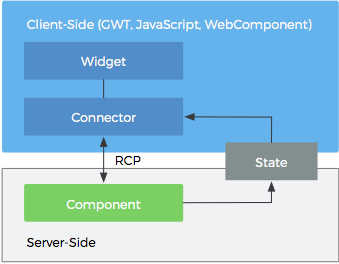
\includegraphics[scale=1.5]{schema.png}
	 				\caption{Esquema Cliente-Servidor}\label{fig:schema}
	 			\end{figure}
 			
	
	
	\section{Spring}
	
		\begin{figure}[H]
			\centering
			
\includegraphics[scale=0.5]{spring.png}
			\caption{Spring Logo}\label{fig:spring}
		\end{figure}
		
		Spring\cite{spring} es un Framework que proporciona un modelo de programación y configuración integral para aplicaciones empresariales modernas basadas en Java y en cualquier tipo de plataforma de implementación. Un elemento clave de Spring es el soporte de infraestructura a nivel de aplicación, ya que Spring se centra abstraer a las aplicaciones empresariales del uso de diferentes frameworks para que los equipos puedan centrarse en la lógica empresarial a nivel de aplicación, sin lazos innecesarios con entornos de implementación específicos.
	
	